% TeX root = main.tex
\section{Fourier Series}

  \subsection{Definition and basic properties}

    We'll begin by reviewing the definition of $L^p$ space since we'll be mostly working on functions from these space.
  \begin{definition}[$L^p$ function]
    \label{Lp_function}
    A real valued function $f$ defined on a lebesgue measurable space $S$ is called an $L^p$ function on $S$ or a $p$-integrable function on $S$ if 
    \begin{displaymath}
       \left( \int_{S} |f(x)|^p \right)^{1/p} < \infty
    \end{displaymath}
\end{definition}  
  Although we've defined general $L^p$ spaces, we'll mostly be concerned about $L^1$ and $L^2$ functions in $\R$ and $\T = [0, 1)$ .
  \\

  Now let's define what a periodic function is.
  \begin{definition}[Periodic function]
    \label{def:periodic_function}
    A function $f:\R \to \R$ is called periodic with period $p$(or $p$-periodic) if $f(x+p) = f(x)$ for all $x \in \R$

  \end{definition}
  Although we're definining real valued periodic functions the definition holds well for any function $f$ from the reals to a space where equality is defined.
  Also note that if we know the value of a $p$ periodic function $f$ in a closed-open (or open-close or closed) interval of length $p$ say $[x, x+p)$, then using the definition of periodic function we can get the function value at the whole of $\R$(we leave it for the reader to verify). That is, we can identify any $p$ periodic function $f$ on $\R$ with the restriction of $f$ onto an interval of length $p$. We can also identify $f$ with the values in a unit circle in $\C$.
  Specifically we'll be working with $1$-periodic functions identified by their restrictions in $\T$.
\\

  Now let's prove an important result of periodic functions.
  \begin{lemma}
    \label{lem:integral_of_periodic_function}
    If $f:\R \to \R$ is of period $1$ and $\int_{0}^{1} f(x) dx$ exists, then for any real number $a$, 
    \begin{displaymath}
      \int_{a}^{a+1}f(x) dx = \int_{0}^{1} f(x) dx
    \end{displaymath} 
  \end{lemma}
  \begin{proof}
    Let $a = n +b$, where $0\le b <1$ and $n$ is an integer. Then since $f$ has period 1,
    \begin{displaymath}
      \int_{a}^{a+1}f(x) dx = \int_{n+b}^{n+b+1}f(x)dx = \int_{b}^{b+1}f(x+n)dx = \int_{b}^{b+1}f(x)dx
    \end{displaymath}
    and, 
    \begin{align*}
      \int_{b}^{b+1}f(x)dx &= \int_{b}^{1}f(x)dx + \int_{1}^{b+1}f(x)dx \\
                      &= \int_{b}^{1}f(x)dx + \int_{0}^{b}f(x+1)dx \\
                      &= \int_{b}^{1}f(x)dx + \int_{0}^{b}f(x)dx \\
                      &= \int_{0}^{1}f(x)dx
    \end{align*}

    Hence the result.
    
  \end{proof}

  Now we'll define fourier coefficients of a periodic function $f \in L^1(\T)$
  \begin{definition}[Fourier coefficient]
    \label{def:fourier_coefficient}
    Let $f \in L^1(\T)$, i.e $\int_{\T} f < \infty$. Then for each integer $n$ we define the $n^{th}$ fourier coefficient, $\hat{f}(n)$ as 
    \begin{displaymath}
      \hat{f}(n) = \int_0^1 f(x)e^{-2\pi inx} dx \end{displaymath}
  \end{definition}
  $\hat{f}(n)$ is finite and well defined for each $n$ since $f \in L^1(\T)$, since
  \begin{displaymath}
    |\hat{f}(n)| \le \int_0^1 |f(x)e^{-2\pi inx}| dx \le \int_0^1 |f(x)||e^{-2\pi inx}| dx = \int_0^1|f(x)| dx < \infty
  \end{displaymath}
  
  Once we have the fourier coefficients of a function at hand we can combine them together to make a series called the fourier series. We'll be investigating the conditions at which this series converges to our initial function $f$.

  \begin{definition}[Fourier series]
    \label{def:fourier_series}
    Given a function $f \in L^1(\T)$, the fourier series of the function $f$ is defined as 
    \begin{displaymath}
      \sum_{n\in \Z} \hat{f}(n)e^{2\pi inx}
    \end{displaymath}
    where $\hat{f}(n)$ is the $n^{th}$ fourier coefficient as defined in \ref{def:fourier_coefficient} 
  \end{definition}

  \begin{theorem}[Properties of Fourier series]
    \label{thm:properties_of_fourier_series}
    Suppose that $f\in L^1(\T)$.
    \begin{enumerate}[label=(\alph*)]
      \item If $a$ is a real number and $g(x) = f(x+a)$ for all $x$, then $\hat{g}(n) = \hat{f}(n)e^{2\pi ina}$ for all $n \in \Z$.
      \item if $b$ is an integer and $h(x) = f(x)e^{2\pi i bx}$ for all $x$, then $\hat{h}(n) = \hat{f}(n-b)$ for all $n\in \Z$.
      \item if $j(x) = f(-x)$ for all $x$, then $\hatj(n) = \hatf(-n)$
    \end{enumerate}
  \end{theorem}
  \begin{proof}
     Given $f(x) \in L^1(\T)$ and $n^{th}$ Fourier coefficient of $f$,  
    \[\hatf(n) = \int_{0}^{1}f(x)e^{-2 \pi inx}.\]
    \begin{enumerate}
      \item[(a)] Then, the $n^{th}$ Fourier coefficient of $g(x) = f(x+a)$ is
        \begin{align*}
          \hatg(n) &= \int_{0}^{1}g(x)e^{-2\pi inx} dx \\
                &= \int_{0}^{1}f(x+a)e^{-2\pi inx} dx \\
                &= \int_{0}^{1}f(x)e^{-2\pi in(x-a)} dx \\
                &= e^{2\pi ina} \int_0^1 f(x)e^{-2\pi inx} dx \\
                &= e^{2\pi ina} \hatf(n)
        \end{align*}

      \item[(b)] If $h(x) = f(x)e^{2\pi ibx}$, then
        \begin{displaymath}
          \hath(n) = \int_0^1 f(x)e^{-2 \pi i (n-b)x} dx = \hatf(n-b)
        \end{displaymath}
      \item[(c)] $j(x) = f(-x)$, then
        \begin{align*}
          \hatj(n)  &= \int_0^1 f(-x)e^{-2\pi inx} dx \\
                    &= -\int_0^{-1} f(y) e^{2\pi iny}dy & \text{by } y=-x\\
                    &= \int_{-1}^0 f(y)e^{2\pi iny}dy \\
                    &= \int_0^1 f(y)e^{2\pi iny}dy & \text{by lemma }\ref{lem:integral_of_periodic_function}\\
                    &= \hatf(-n)
        \end{align*}
        
        
    \end{enumerate}
  \end{proof}


  \subsection{Convolution}
  Now we'll define another important operation with function called the convolution of two functions.
  \begin{definition}
    Let $f, g \in L^1(\T)$, then the convolution of $f$ and $g$ is defined as 
    \begin{displaymath}
      f*g(x) = \int_0^1 f(y)g(x-y)dy
    \end{displaymath}
  \end{definition}

  Convolution can be thought of as taking the moving average of a function with another function. Refer figure \ref{fig:convolution}.
  \begin{figure}
    \centering
    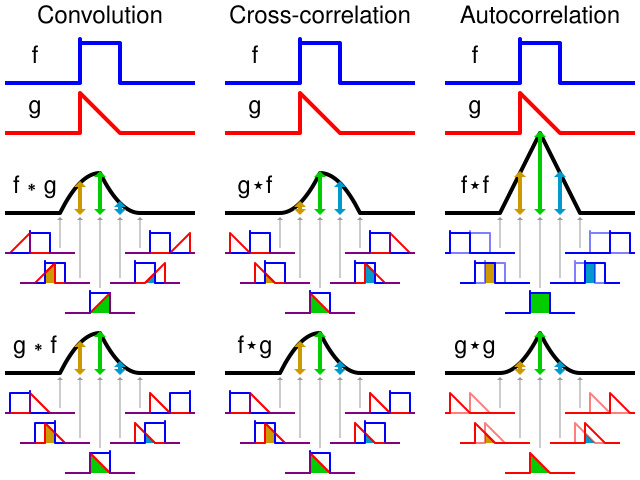
\includegraphics[width=0.6\textwidth]{convolution}
    \caption{convolution}
    \label{fig:convolution}
  \end{figure}

  \begin{proposition}[Properties of convolution]
    \label{prop:properties_of_convolution}
    Let $f, g \in L^1(\T)$, then 
    \begin{enumerate}[label=(\alph*)]
      \item $f*g = g*f$
      \item $f*(g+h) = f*g +f*h$
      \item $(cf)*g = c(f*g)$
      \item $f*(g*h) = (f*g)*h$
    \end{enumerate}
  \end{proposition}
  \begin{proof}
    We'll just prove the commutativity and will leave the rest for the reader to verify. (Hint: Use properties of integration)

    Put $v = x-y$, we get $dv = -dy$ and 
    \begin{align*}
      f*g(x)  &= \int_{0}^{1}f(y)g(x-y) dy \\
              &= -\int_{x}^{x-1} f(x - v)g(v) dy\\
              &= \int_{x-1}^{x} g(v)f(x-v) dy \\
              &= \int_{0}^{1}g(v)f(x-v)dy  &\text{by lemma } \ref{lem:integral_of_periodic_function}\\
              &=g*f(x)
    \end{align*} 
  \end{proof}
  

  We'll prove another important result that the convolution of two $L^1(\T)$ functions is again in $L^1(\T)$.
  \begin{theorem}
    \label{thm:convolution_is_in_L1}
  Let $f, g \in L^1(\T)$. Then $h = f*g \in L^1(\T)$, and $\hath(n) = \hatf(n)\hatg(n)$.
  \end{theorem}
  % \begin{proof}
  %   Consider the function $h: \T^2 \to \T$ defined as $h(x, y) = f(x)$. Then
  %   \begin{align*}
  %     h^{-1}(a, 1) &= \{(x, y)\in \T^2, h(x,y) > a \} \\
  %                 &= \{(x, y)\in \T^2, f(x) > a \} \\
  %                 &= f^{-1}(a, 1)\times \T
  %   \end{align*}
  %   Similarly, define $k(x, y): \T^2 \to \T$ as $k(x, y) = g(y)$. Then we'll get $k^{-1}(b, 1) = \T \times g^{-1}(b, 1)$ like above. 
  %   Since $f, g$ are measurable functions in $\T$, $f^{-1}(a, 1), g^{-1}(b, 1)$ are measurable sets in $\T$ and hence $h, k$ are measurable functions in $\T^2$.
  %   
  %   Then $F(x, y): \T^2 \to \T$ defined as $F(x, y) = f(x)g(y)$ is a measurable function, since $F^{-1}((a, b)\times (c, d)) = f^{-1}(a, b) \times g^{-1}(c, d)$ which is again open for any open set $(a, b)\times (c, d)$ in $\T^2$
  %
  %   Again $T: \T^2 \to \T$ defined as $T(x, y) = (x,x-y)$ is measurable being linear. Hence $H: \T^2 \to \T$ defined as $H(x, y) = F \circ T (x, y) = f(x)g(x-y)$ is measurable being the composition of measurable functions. 
  %   
  % \end{proof}

  \begin{proof}
    \begin{align*}
  \int_{0}^{1} |h(x)| dx &= \int_{0}^{1} \left| \int_{0}^{1} f(y)g(x-y)\  dy \right| dx \\
                         &\le \int_{0}^{1} \int_{0}^{1} |f(y)g(x-y)| \ dy \ dx \\
                         &= \int_{0}^{1} \int_{0}^{1} |f(y)g(x-y)| \ dx \ dy & \text{by Tonelli's theorem}\\
                         &= \int_{0}^{1} \left( \int_{0}^{1} |g(x-y)| dx \right) |f(y)|dy \\
                         &=\norm{f}_1 \norm{g}_1
    \end{align*}

    Note that we're using Tonelli's theorem here to interchange the limits of integration since the space is a finite measure space. This proves that $h = f*g \in L^1(\T)$.

    To prove the next part,
    \begin{align*}
      \hath(n) &= \int_0^1 \left( \int_0^1 f(y)g(x-y)dy \right) e^{-2\pi in x} dx \\
               &= \int_0^1 f(y) \left( \int_0^1 g(x-y) e^{-2\pi in x}dx \right) dy & \text{by Tonelli's theorem}\\  
               &= \int_0^1 f(y) \hatg(n)e^{-2\pi inx} dy & \text{by theorem } \ref{thm:properties_of_fourier_series} \text{(a)}\\
               &= \hatf(n)\hatg(n)
    \end{align*}
  \end{proof}
 

  \subsection{Summability of Fourier series}
  Given a function $f$ in the $\T$, we are interested in the convergence of fourier series of $f$. We'll discuss about the convergence of the symmetric partial sum of the Fourier series.

  \begin{definition}[Symmetric partial sum of a Fourier series]
    \label{def:symmetric_partial_sum_of_fourier_series}
    Given a function $f \in \L^1(\T)$ with its fourier series, $\sum_{-\infty}^\infty \hatf(n)e^{2\pi in x}$, we define the $n^{th}$ symmetric parial sum of the fourier series as
    \begin{displaymath}
      S_N(x) = \sum_{n=-N}^N \hatf(n)e^{2\pi inx}
    \end{displaymath}
  \end{definition}
  But it may happen that the summetric partial sum of the Fourier seies may not converge. To deal with this we'll define another partial sum called the Ces\'aro partial sum.

  \begin{definition}[Ces\'aro partial sum of Fourier series]
    \label{def:cesaro_partial_sum_of_fourier_series}
    Given a function $f \in \L^1(\T)$ with its Fourier series, $\sum_{-\infty}^\infty \hatf(n)e^{2\pi in x}$, we define the $n^{th}$ Ces\'aro parial sum of its Fourier series as
    \begin{displaymath}
      \sigma_N(x) = \frac{1}{N}\sum_{n=0}^{N-1} S_n(x)
    \end{displaymath}
    where $S_n(x)$ is the symmetric partial sum of the Fourier series as defined in \ref{def:symmetric_partial_sum_of_fourier_series}
  \end{definition}
  For an example, $\{-1^{n}\}$ is a sequence whose symmetric partial sums do not converge but the Ces\'aro partial sums converge to $\frac{1}{2}$. Also if the symmetric partial sums of a series converge, then the Ces\'aro partial sums will also converge to the same limit. \textcolor{red}{(Prove it!)}

  Now we'll show that the Ces\'aro partial sum can be rewritten to another form which will help our proofs down the road.
  \begin{lemma}
    \label{lem:property_of_cesaro_partial_sum}
    If $\sigma_N(x)$ is the $N^{th}$ Ces\'aro partial sum of the Fourier series of a function $f\in L^1(\T)$, then
    \begin{displaymath}
      \sigma_N(x) = \sum_{n=-N}^N \left(1-\frac{\abs{n}}{N} \right) \hatf(n) e^{2\pi inx}
    \end{displaymath}
  \end{lemma}
  \begin{proof}
    We'll prove the result for a general series so that it'll help us also in Fourier series.

    Let $S_N = \sum_{n=-N}^{N}a_n$ be the $N^{th}$ partial sum of the series $\sum_{-\infty}^{\infty}a_n$. Then by the definition of Ces\'aro partial sum, 
    \begin{align*}
      \sigma_N  &= \frac{1}{N} \sum_{n=0}^{N-1}S_n \\
                &= \frac{1}{N} \sum_{n=0}^{N-1}\sum_{k=-n}^{n}a_k \\
                &= \frac{1}{N} \sum_{k=-N+1}^{N-1} a_k \sum_{n=|k|}^{N-1} 1 \\
                &= \frac{1}{N} \sum_{k=-N+1}^{N-1} \left(N - |k|\right) a_k \\
                &=  \sum_{k=-N+1}^{N-1} \left(1 - \frac{|k|}{N}\right) a_k \\
                &=  \sum_{k=-N}^{N} \left(1 - \frac{|k|}{N}\right) a_k \\ 
    \end{align*}
    Now speficially if we take $a_k = \hatf(k)e^{2\pi ikx}$, we get the required result. 
  \end{proof}

  For that we'll use a collection of function called the summability kernels
  \begin{definition}[Summability kernel]
    \label{def:summability_kernel}
    A sequence of functions $K_N \in L^1(\T)$ is called a summability kernel or an approximation identity if 
    \begin{enumerate}[label=(\alph*)]
      \item $\int_{0}^{1}K_N(x)dx = 1$
      \item $\int_{0}^{1}\abs{K_N(x)}dx \le C$ for some constant $C>0$
      \item $\lim_{N\to\infty} \int_{\delta}^{1-\delta}\abs{K_N(x)}dx= 0$
    \end{enumerate}
  \end{definition}
 

  Now we'll define one of the important summability kernels.
  \begin{definition}[Fej\'er kernel]
    \label{def:fejer_kernel}
    Fej\'er kernel is defined as a collection of functions  $\Delta_N$ where for each $N \in \N$, $\Delta_N : \R \to \R$ is defined as 
    \begin{displaymath}
      \Delta_N(x) = \sum_{n=-N}^{N}\left( 1 - \frac{\abs{n}}{N}\right)e^{2\pi inx}
    \end{displaymath}
  \end{definition}
  Notice that each $\Delta_N$ is a $1-$periodic function.

  We'll prove that Fej\'er kernel as defined in \ref{def:fejer_kernel} satify the properties in \ref{def:summability_kernel}. But before that we'll explore some properties of Fej\'er kernel so that it'll aid us in our proof.
  \begin{proposition}[Properties of Fej\'er kernel]
    \label{prop:properties_of_fejer_kernel}
    If $\Delta_N(x)$ is defined as in \ref{def:fejer_kernel}, then the following hold true
    \begin{enumerate}[label=(\alph*)]
      \item
        \begin{displaymath}
          \Delta_N(x) = 
            \begin{cases}
              \frac{1}{N}\left( \frac{\sin(\pi Nx)}{\sin(\pi x)} \right)^2, \quad \text{if } x\notin \Z \\
              N, \quad \text{if } n \in \Z\
            \end{cases}
        \end{displaymath}
      \item 
        \begin{displaymath}
          (\Delta_N*f)(x) = \sigma_N(x) 
        \end{displaymath}
        where $\sigma_n(x)$ is the $n^{th}$ Ces\'aro partial sum of the Fourier series of $f$ as defined in $\ref{def:cesaro_partial_sum_of_fourier_series}$
    \end{enumerate}
  \end{proposition}

  \begin{proof}
    \begin{enumerate}[label=(\alph*)]
      \item
        If $x\in \N$ then $e^{2\pi inx} = 1$ for all $n$ and then,
        \begin{displaymath}
          \sum_{n=0}^{N-1}e^{2\pi inx} = \sum_{n=0}^{N-1} 1 = N
        \end{displaymath}
        Hence the last case is solved. But if $x\notin \N$ then from the finite sum of geometric series,
        \begin{align*}
          \sum_{n=0}^{N-1}e^{2\pi inx} &= \frac{e^{2\pi iNx} - 1}{e^{2\pi ix} - 1} \\
                  & = \frac{e^{\pi iNx}}{e^{\pi ix}} \frac{e^{\pi iNx} - e^{-\pi iNx}}{e^{\pi ix} - e^{-\pi ix}} \\
                  & = e^{\pi i(N-1)x}\frac{\sin(\pi Nx)}{\sin(\pi x)}
        \end{align*}
        Since $\abs{e^{ix}} = 1$ for all $x\in \R$, we'll get
        \begin{displaymath}
          \left|\sum_{n=0}^{N-1}e^{2 \pi inx}\right|^2 = \frac{\sin^2(\pi Nx)}{\sin^2{\pi x}}  
        \end{displaymath}

        But we also know that,
        \begin{align*}
         \left|\sum_{n=0}^{N-1}e^{2 \pi inx}\right|^2 &= \left(\sum_{n=0}^{N-1}e^{2 \pi inx}\right)  \left(\sum_{n=0}^{N-1}\overline{e^{2 \pi inx}}\right) \\
            &= \sum_{m=0}^{N-1} \sum_{n=0}^{N-1} e^{2\pi i(m-n)x} \\
            &= \sum_{k = -(N-1)}^{N-1} e^{2\pi ikx} \sum_{\substack{0\le m \le N-1 \\ 0 \le n \le N-1 \\ m-n = k}}1 \\
            &= \sum_{k = -(N-1)}^{N-1} e^{2\pi ikx} (N - |k|) \\
            &= N\Delta_N(x)
        \end{align*}

        Which implies that 
        \begin{displaymath}
          \Delta_N(x) = \frac{1}{N}\frac{\sin^2(\pi Nx)}{\sin^2{\pi x}}
        \end{displaymath}
      Hence the proposition.

    \item
      \begin{align*}
        (\Delta_N*f)(x) &= \int_0^1 \Delta_N(y)f(x-y) \ dy \\
              &= \int_0^1 \sum_{n=-N}^{N} \left(1-\frac{\abs{n}}{N}\right)e^{2\pi iny} f(x-y) \ dy \\
              &= \sum_{n=-N}^N  \left(1-\frac{\abs{n}}{N}\right) \int_0^1 f(x-y) e^{2\pi iny} \ dy \\
              &= \sum_{n=-N}^N  \left(1-\frac{\abs{n}}{N}\right) e^{2 \pi inx}  \int_0^1 f(x-y) e^{-2\pi in \left( x-y \right) } \ dy \\
              &= \sum_{n=-N}^N  \left(1-\frac{\abs{n}}{N}\right) e^{2 \pi inx} \int_x^{x-1} -f(v) e^{-2\pi in v} \ dv \\
              &= \sum_{n=-N}^N  \left(1-\frac{\abs{n}}{N}\right) e^{2 \pi inx} \int_{x-1}^x f(v) e^{-2\pi in v} \ dv \\
              &= \sum_{n=-N}^N  \left(1-\frac{\abs{n}}{N}\right) e^{2 \pi inx} \int_0^{1} f(v) e^{-2\pi in v} \ dv & \text{by lemma } \ref{lem:integral_of_periodic_function}\\
              &= \sum_{n=-N}^N  \left(1-\frac{\abs{n}}{N}\right) e^{2 \pi inx} \hatf(n) \\
              &= \sigma_N(x)
      \end{align*}
    \end{enumerate}
\end{proof}
  

  \begin{proposition}
    \label{prop:fejer_kernel_is_summability_kernel}
    Fej\'er kernel as defined in \ref{def:fejer_kernel} is a summability kernel as in definition \ref{def:summability_kernel}
  \end{proposition}
  \begin{proof}
    \begin{enumerate}[label=(\alph*)]
      \item
        By definition,
        \begin{align*}
          \Delta_N(x) &= \sum_{n=-N}^{N}\left(1-\frac{\abs{n}}{N}\right)e^{2\pi inx} \\
                      &= 1 + 2\sum_{n=1}^N \left(1-\frac{|n|}{N}\right)\cos(2\pi nx) \\
        \end{align*}
        Therefore, 
        \begin{align*}
          \int_0^1\Delta_N(x) \ dx &= \int_0^1 1\ dx + 2\sum_{n=1}^N \left(1 - \frac{|n|}{N}\right)\int_0^1cos(2\pi nx) \ dx \\
                &= 1 + 0 \\ 
        \end{align*}
        This proves the first statement in the definition of summability kernel in \ref{def:summability_kernel}

      \item
        Since $\Delta_N(x) \ge 0$ for all $x\in \R$, by \ref{prop:properties_of_fejer_kernel}
        \begin{displaymath}
          \int_0^1 \left|\Delta_N(x)\right| dx = \int_0^1 \Delta(x) dx = 1
        \end{displaymath}
        This proves the $2^{nd}$ condition for the summability kernel.
        
      \item
        To prove that 
        \begin{displaymath}
          \lim_{N \to \infty}\int_\delta^{1-\delta} \left|\Delta_N(x) \right| dx = 0
        \end{displaymath}
        we'll first see that $\sin(\pi x) \ge 2x$ whenever $0\le x\le \frac{1}{2}$. 
        But this is because the $f(x) := \sin(\pi x) - 2x = 0$ only for $x=0$ and $x=2$ and the derivative of $f$, $f'(x) := \pi \cos(\pi x) - 2 = 0$, only for a unique real number $r\in [0, \frac{1}{2}]$.Now since $f$ is smooth, $f$ cannot have more roots in $[0, \frac{1}{2}]$. Hence $\sin(\pi x) \ge 2x$ for all $x \in [0, \frac{1}{2}]$

        Now we'll get to the main proof. Assume $0 < \delta < \frac{1}{2}$. Then by \ref{prop:properties_of_fejer_kernel}
       \begin{align*}
         \Delta_N(x) &= \frac{1}{N}\left(\frac{\sin(\pi Nx)}{\sin(\pi x)}\right)^2 \\
                &\le \frac{1}{N\sin^2(\pi x)} \\
                &\le \frac{1}{4Nx^2} &\text{since } \sin(\pi x) \ge 2x \\
       \end{align*}
        Which implies
        \begin{displaymath}
          \int_\delta^\frac{1}{2} \left| \Delta_N(x) \right| dx \le \int_\delta^\frac{1}{2} \frac{1}{4Nx^2} dx \le \int_\delta^\infty \frac{1}{4Nx^2} dx = \frac{1}{4N\delta}
        \end{displaymath}

        Also note that $\sin^2(\pi N(1-x)) = \sin^2(\pi Nx)$ since,
        \begin{align*}
          \sin(\pi N(1-x))  &= \sin(\pi N - \pi Nx) \\
                            &= \sin( \pi N)\cos(\pi Nx) - \cos(\pi N)\sin(\pi Nx) \\
                            &= 0 - \cos(\pi N)\sin(\pi Nx) & \sin(\pi N) = 0\\
                            &= \pm \sin(\pi Nx)
        \end{align*}

        Therefore $\Delta_N(1-x) = \Delta_N(x)$ and 
        \begin{align*}
          \int_\frac{1}{2}^{1-\delta} \Delta_N(x) &= \int_\frac{1}{2}^{1-\delta} \Delta_N(1-x)  \\
                &= -\int_\frac{1}{2}^\delta \Delta_N(x) & \text{change of variables} \\
                &=  \int_\delta^\frac{1}{2} \Delta_N(x)
        \end{align*}

        Hence,
        \begin{displaymath}
          \int_\delta^{1-\delta} \Delta_N(x) = \int_\delta^\frac{1}{2} \Delta_N(x) + \int_\frac{1}{2}^\delta \Delta_N(x) \le 2 \int_\delta^\frac{1}{2} \Delta_N(x) \le \frac{1}{2N\delta}
        \end{displaymath}
       
        Therefore, for $0 < \delta < \frac{1}{2}$, we have 
        \begin{displaymath}
          \lim_{N \to \infty} \int_\delta^{1-\delta} \left|\Delta_N(x)\right| = \lim_{N \to \infty} \int_\delta^{1-\delta} \Delta_N(x) = 0
        \end{displaymath}

        If $\frac{1}{2} < \delta < 1$ then by change of variable $y = 1 - x$
        \begin{displaymath}
          \int_\delta^{1-\delta} \Delta_n(x) =  - \int_{1-\delta}^{\delta} \Delta_n(y) = 0
        \end{displaymath}
        And therefore for all $0 < \delta < 1$ 
        \begin{displaymath}
          \lim_{N \to \infty} \int_\delta^{1-\delta} \left|\Delta_N(x)\right| =  0
        \end{displaymath}


      Which completes the proof that  Feje\'r kernel is a summability kernel.
    \end{enumerate}
  \end{proof}



  Now we prove an important theorem which will serve as a backbone for the discussion of convergence forward.
  \begin{theorem}[Convergence to convolution of summability kernels]
    \label{thm:L1_convergence_of_summability_kernel}
    If $f\in L^1(\T)$ and $K_N$ is a summability kernel then $f*K_N$ converges to $f$ in $L^1$ norm. That is
    \begin{displaymath}
      \lim_{N\to \infty} \int_{0}^{1}\abs{f(x) - (f*K_N)(x))} = 0
    \end{displaymath}
\end{theorem}
  \begin{proof}
    \begin{displaymath}
      f*K_N(x) = \int_0^1 f(x-y)K_N(x)dx
    \end{displaymath}
    Since $\int_0^1 K_N(y)dy = 1$, by the $2^{nd}$ property of summability kernel,
    \begin{displaymath}
      f(x) - f*K_N(x) = \int_0^1\left(f(x)-f(x-y)\right)K_N(y)dx
    \end{displaymath}
    Now then, 
    \begin{align*}
      \int_0^1 |f(x) - K_N(x)| dx &= \int_0^1 \left| \int_0^1 (f(x) - f(x-y))K_N(y)dy \ \right| \ dx \\
                &\le \int_0^1 \int_0^1 \left| f(x) - f(x-y) K_N(y) \right| dy \ dx \\
                &= \int_0^1 |K_N(y)| \int_0^1 |f(x) - f(x-y)| dx \ dy & \text{by Tonelli's theorem} \\
                &= \int_{-\delta}^{1-\delta} & \text{by lemma } \ref{lem:integral_of_periodic_function} \\
                &= \int_{-\delta}^{\delta} + \int_{\delta}^{1-\delta} = I_1 + I_2\\
    \end{align*}
    We'll show that for a given $\epsilon$ we can find an $N$ such that for all $n>N, \ I_1+I_2 < \epsilon$

    Since $f \in L^1(\T)$ we can find $\delta >0$ such that $\int_0^1| f(x+\delta) - f(x) | dx = \epsilon / 2C$, where $C$ is the constant in the second conditon of summability kernel. The proof can be found in any measure theory textbook.
    
    Then, 
    \begin{displaymath}
      |I_1| \le \frac{\epsilon}{2C} \int_{-\delta}^{\delta}|K_N(y)|dy \le \frac{\epsilon}{2C} \int_0^1 |K_N(y)| dy \le \frac{\epsilon}{2}
    \end{displaymath}  
    
    For $I_2$, we see that 
    \begin{displaymath}
      \int_0^1 |f(x) - f(x-y)|dx \le \int_0^1 |f(x)| dx + \int_0^1 |f(x-y)| dx = 2\norm{f}_1
    \end{displaymath}
  Then,
  \begin{displaymath}
    |I_2| \le 2\norm{f}_1 \int_{\delta}^{1-\delta} |K_N(y)|dy
  \end{displaymath}
But by the $3^{rd}$ property of the summability kernel, we know that the integral in the above converges to zero. Therefore there exists an $N$ such that for ann $n>N, |I_2|< \epsilon/2$, which completes our proof.
  \end{proof}

  \begin{corollary}{Convergence of Ces\'aro sum of functions in $L^1(\T)$}
    If $f\in L^(\T)$ then $\sigma_N(x)$, the Ces\'aro sum of the Fourier series of $f$ converge to $f(x)$ in $L^1$ norm. That is, 
    \begin{displaymath}
      \lim_{N\to \infty} \int_0^1 \left|f(x) - \sigma_N(x)\right| = 0
    \end{displaymath}
  \end{corollary}
  \begin{proof}
    Since we know that Fej\'er kernel, $\Delta_N(x)$ is a summability kernel by proposition \ref{prop:fejer_kernel_is_summability_kernel} and that $(\Delta_N*f)(x) = \sigma_N(x)$ by prop \ref{prop:properties_of_fejer_kernel}, the result follows from theorem \ref{thm:L1_convergence_of_summability_kernel}.
  \end{proof}
  
